Una vez definida la funcionalidad base de la aplicación y para mejorar la apariencia de ésta, haciendo más fácil y visual su uso, se han realizado múltiples modificaciones mediante el uso de \textit{Property nodes} principalmente, aunque también se han utilizado otros recursos.

Se ha creado un indicador personalizado\cite{customcontrol} para mostrar una imagen en formato PNG con transparencia. Esta imagen corresponde al logotipo del proyecto que puede verse en la figura \ref{fig:acher_front}. No es ésta la forma más elegante de mostrar una imagen estática, pues para eso se dispone de otros recursos específicos, pero ha resultado la más fácil y rápida desde el punto de vista del desarrollador. Se ha modificado un indicador de tipo booleano para que muestre la misma imagen independientemente del valor que se le asigne. Este indicador puede encontrarse con el nombre \textit{logo\_acher.ctl} entre las fuentes del proyecto.

El controlador de tipo string que define el contenido a enviar por la aplicación se ha configurado mediante \textit{Property nodes} para que el texto aparezca siempre centrado y el tamaño sea mayor que el que aparece por defecto. Estos parámetros son constantes, por lo que el usuario no puede modificarlos durante la ejecución.

\begin{figure}[!htp]
\centering
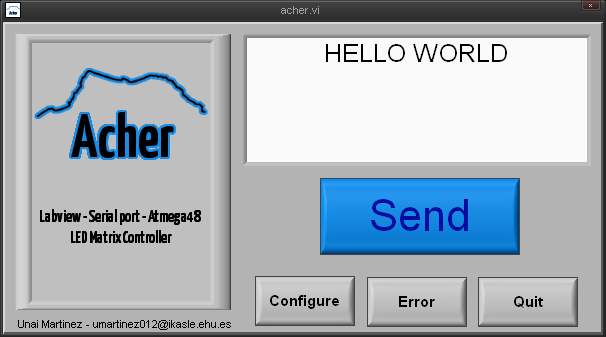
\includegraphics[width=300pt]{./images/acher_front.png}
\caption{Panel frontal: vista general.}
\label{fig:acher_front}
\end{figure}

Se han creado cuatro botones (controladores booleanos) para que el usuario pueda interactuar con la aplicación. Éstos son \textit{Send}, \textit{Configure}, \textit{Error} y \textit{Quit}.

\begin{itemize}

\item{\textbf{Send}:

La función de este botón es enviar, al pulsar sobre él, el contenido del controlador de tipo string:

Todo el programa se encuentra dentro de un bucle \textit{while}. El valor del botón \textit{Send} controla una estructura \textit{case} dentro del \textit{while}. Cuando es verdadera, se ejecuta la aplicación base analizada en la sección anterior. Mientras sea falsa, no se ejecuta acción ninguna.

Mediante los \textit{Property nodes} se han modificado el tamaño y color del texto y el color de fondo del botón. Este último, además, cambia cuando el botón está pulsado. El texto se encuentra en todo momento centrado tanto vertical como horizontalmente.
}

\item{\textbf{Configure}:

Este botón muestra y oculta los controladores que definen los parámetros a utilizar por el bloque \textit{VISA Configure Serial Port}. Para ello, actúa sobre la propiedad de visibilidad de éstos, además de sobre la misma propiedad del indicador utilizado para mostrar el logotipo y el \textit{Simple Error Handler}. También afecta al parámetro \textit{Disabled} del controlador string, del botón \textit{Send} y del botón \textit{Error}.

\begin{figure}[!htp]
\centering
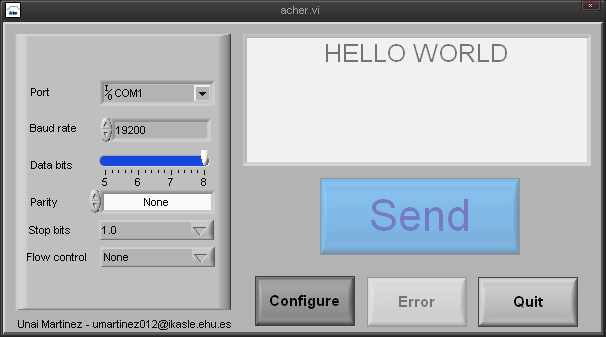
\includegraphics[width=275pt]{./images/acher_config.png}
\caption{Panel frontal: configure.}
\label{fig:acher_config}
\end{figure}

De esta manera, cuando el botón se encuentra pulsado y por lo tanto su valor es verdadero (Figura \ref{fig:acher_config}), se muestran únicamente los controladores de configuración, deshabilitando el controlador string y los botones \textit{Send} y \textit{Error}. El logo y el gestor de error se ocultan. Una vez el usuario ha realizado las modificaciones oportunas, la desactivación del botón \textit{Configure} devuelve la aplicación al estado mostrado en la vista general (Figura \ref{fig:acher_front}).

El tamaño del texto del botón y su alineación tanto horizontal como vertical se encuentran definidas mediante constantes.
}

\item{\textbf{Error}:

\begin{figure}[!htp]
\centering
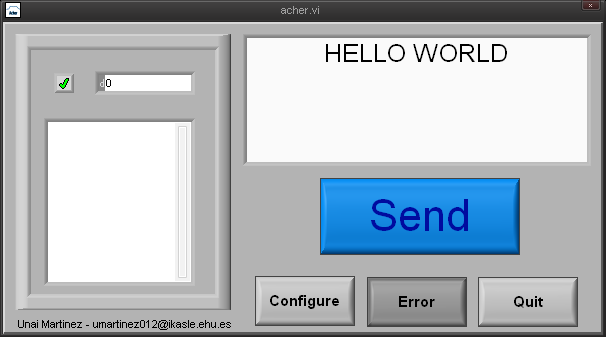
\includegraphics[width=275pt]{./images/acher_err1.png}
\caption{Panel frontal: no error.}
\label{fig:acher_err1}
\end{figure}

El funcionamiento de este botón, muy parecido al de \textit{Configure}, simplemente oculta el logo y muestra el gestor de errores cuando se encuentra pulsado (Figura \ref{fig:acher_err1}). Se debe tener en cuenta que \textit{Configure} tiene prioridad sobre \textit{Error}, por lo que el primero deberá estar desactivado para poder ver el gestor de errores.

El tamaño del texto del botón y su alineación tanto horizontal como vertical se encuentran definidas mediante constantes y mantienen su valor durante toda la ejecución. No así el color de fondo. Cuando se detecta algún error en el envío, éste cambia a rojo (Figura \ref{fig:acher_err2}), indicando así que no se ha efectuado correctamente.

\begin{figure}[!htp]
\centering
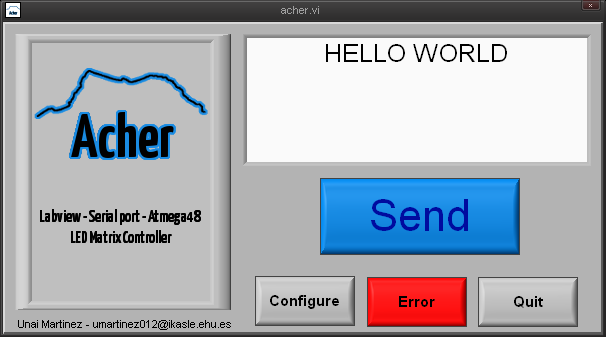
\includegraphics[width=275pt]{./images/acher_err2.png}
\caption{Panel frontal: error.}
\label{fig:acher_err2}
\end{figure}

Pulsando sobre el botón, se puede ver cuál es el error (Figura \ref{fig:acher_err3}). Para diferenciar cuándo se encuentra pulsado y cuándo no, en la nueva definición de color se han especificado dos constantes diferentes, siendo el segundo ligeramente más oscuro. Un simple \textit{select} controlado por el estado del botón booleando \textit{Error} decide cuál utilizar.

\begin{figure}[!htp]
\centering
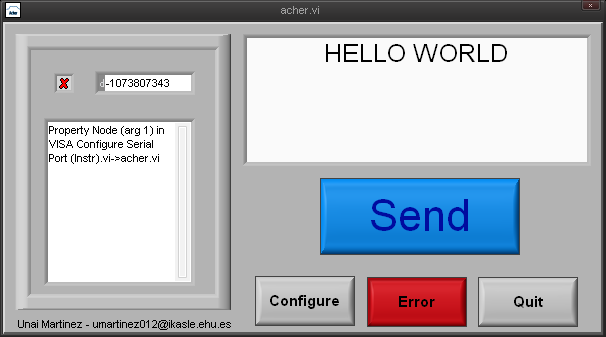
\includegraphics[width=275pt]{./images/acher_err3.png}
\caption{Panel frontal: view error.}
\label{fig:acher_err3}
\end{figure}
}

Al realizar un nuevo envío correcto, y por lo tanto no haber ningún error en el gestor de errores, el botón adquiere de nuevo el color original.

\item{\textbf{Quit}:

Para evitar que el usuario salga de la aplicación por error, la pulsación del botón \textit{Quit} controla una estructura \textit{case}. Cuando el valor es falso, éste se pasa directamente al controlador que termina el bucle \textit{while}, permitiendo que la aplicación siga ejecutándose. Cuando es verdadero, se lanza una ventana que pide confirmación al usuario (Figura \ref{fig:acher_quit}).

\begin{figure}[!htp]
\centering
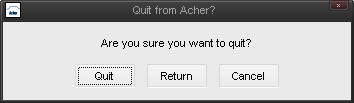
\includegraphics[width=175pt]{./images/acher_quit.png}
\caption{Ventana de salida.}
\label{fig:acher_quit}
\end{figure}

El lanzamiento de esta ventana se efectúa mediante el bloque \textit{Three Button Dialog}. Éste recibe como parámetros el contenido de los tres botones, el título de la ventana, el texto a mostrar y la alineación (Figura \ref{fig:acher_quitcase}). Un bloque de comparación hace que la salida sólo sea verdadera cuando el usuario pulse sobre el botón de la izquierda (\textit{Quit}). Cualquiera de las otras opciones (\textit{Return} o \textit{Cancel}), devolverá una salida falsa, permitiendo que se siga ejecutando el bucle principal.

\begin{figure}[!htp]
\centering
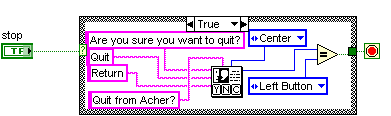
\includegraphics[width=225pt]{./images/acher_quitcase.png}
\caption{Lógica de salida.}
\label{fig:acher_quitcase}
\end{figure}
}

\end{itemize}